\section{Experiments and Performance Evaluation}\label{performance-evaluation}

We designed topologies based on our previous testbed validation. The new
coponent is software router which make virtual host in mininet a router.
In our performance evaluation, all software routers are running OSPF
routing protocols and we want to prove that our testbed can maintain
good performance when adding non-SDN components into our
hardware-in-the-loop SDN testbed.

\subsection{One Mininet}\label{one-mininet}

\subsubsection{Two-way Topology(OneMininet):}\label{two-way-topologyone-mininet}

Two-way test is the basic experiment to validate the fidelity of our
Mininet-Quagga testbed. We conduct a two-way perf test on a simple
topology to check the impact of non-SDN components (Quagga router) in
SDN network.

\begin{figure}[h]
\centering
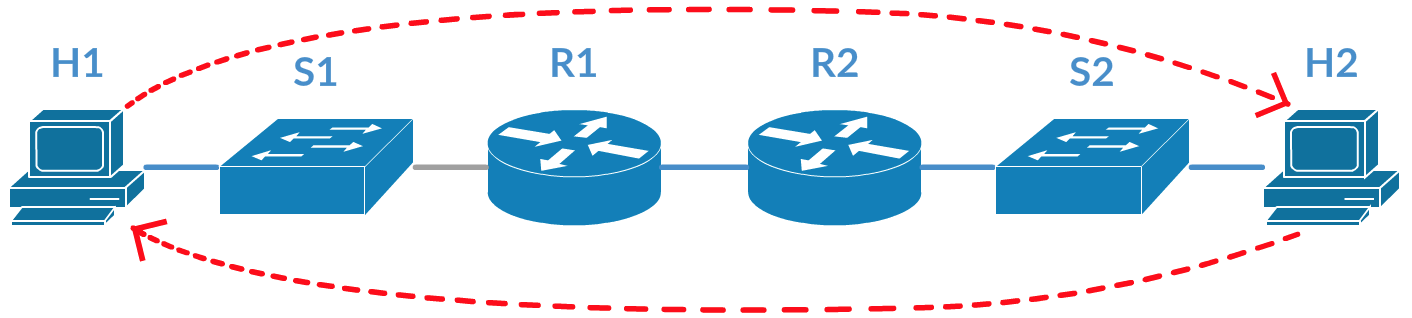
\includegraphics[width=0.7\textwidth]{./Figure/OneMininet(SDN+NONSDN)/Twoway/Twoway(OneMininet).png}
\caption{Two-way Topology(OneMininet) \label{fig:Twoway(OneMininet)}}
\end{figure}

\begin{figure}[h]
\centering
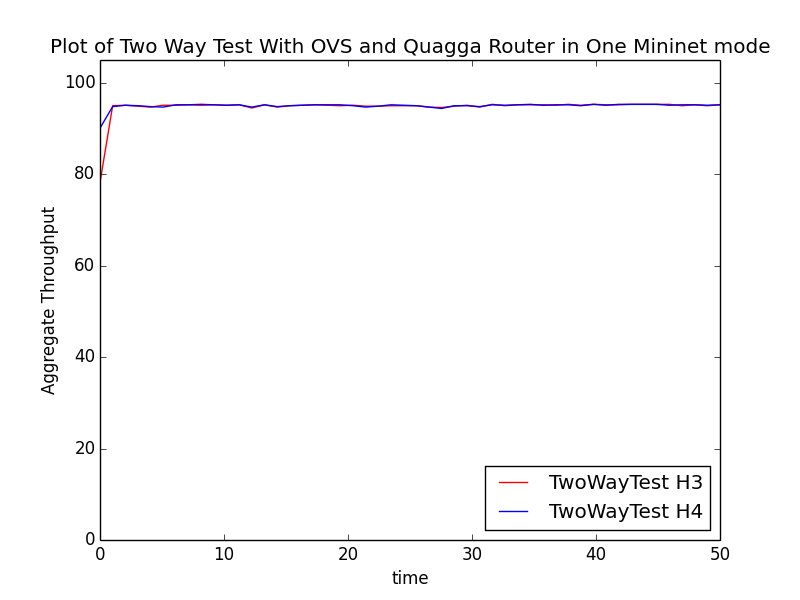
\includegraphics[width=0.6\textwidth]{./Figure/OneMininet(SDN+NONSDN)/Twoway/test.png}
\end{figure}


From the result we can see both connections have an average throughput
above 90 Mbits/sec.

\subsubsection{Fork-in Topology:}\label{fork-in-topology}

We did fork-in test to evaluate the in-boud traffic queuing processing
performance of Quagga routers.

\begin{figure}[h]
\centering
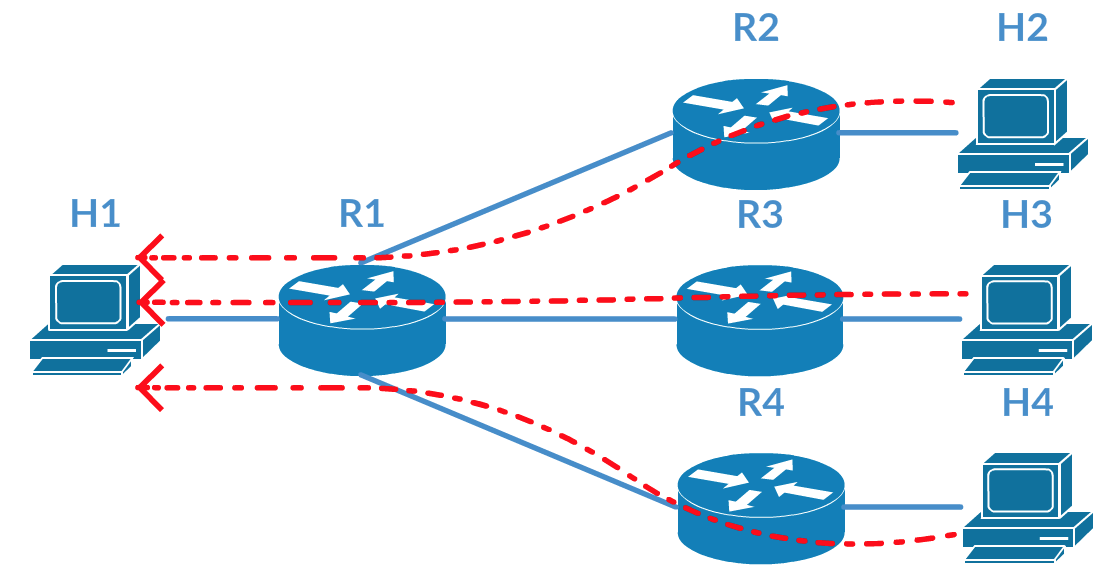
\includegraphics[width=0.7\textwidth]{./Figure/OneMininet(SDN+NONSDN)/ForkIn/ForkIn(OneMininet).png}
\caption{Fork-in Topology \label{fig:Fork-in Topology}}
\end{figure}

\begin{figure}[h]
\centering
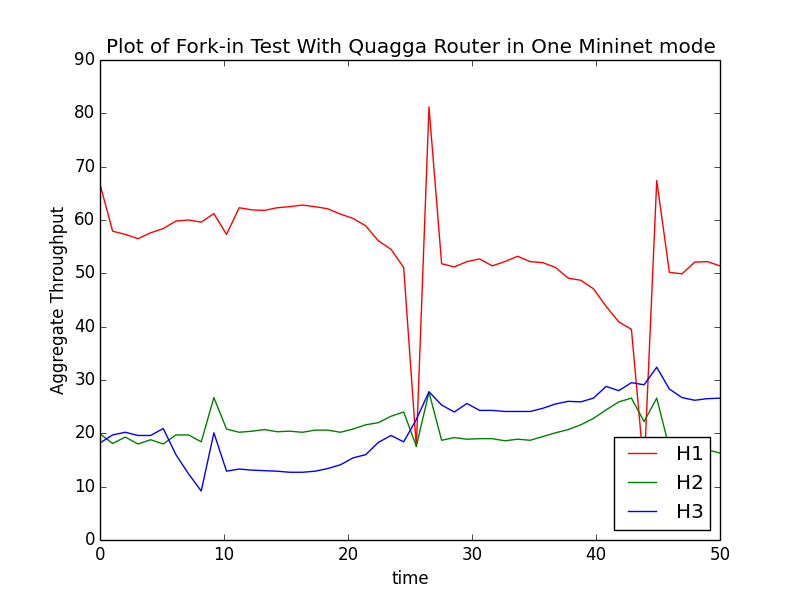
\includegraphics[width=0.6\textwidth]{./Figure/OneMininet(SDN+NONSDN)/ForkIn/ForkIn2.png}
\end{figure}

\subsubsection{Fork-out Topology:}\label{fork-out-topology}

Fork-out test aims to check whether Quagga router can make out-boud
traffic get a fair share of bandwdith resources.

\begin{figure}[h]
\centering
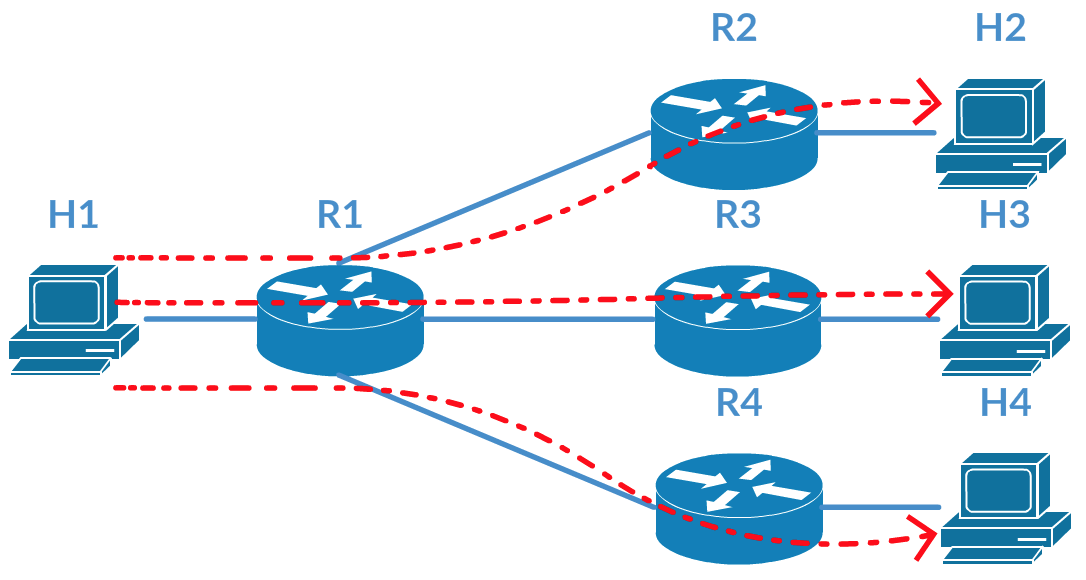
\includegraphics[width=0.7\textwidth]{./Figure/OneMininet(SDN+NONSDN)/ForkOut/ForkOut(OneMininet).png}
\caption{Fork-out Topology \label{fig:Fork-out Topology}}
\end{figure}

\begin{figure}[h]
\centering
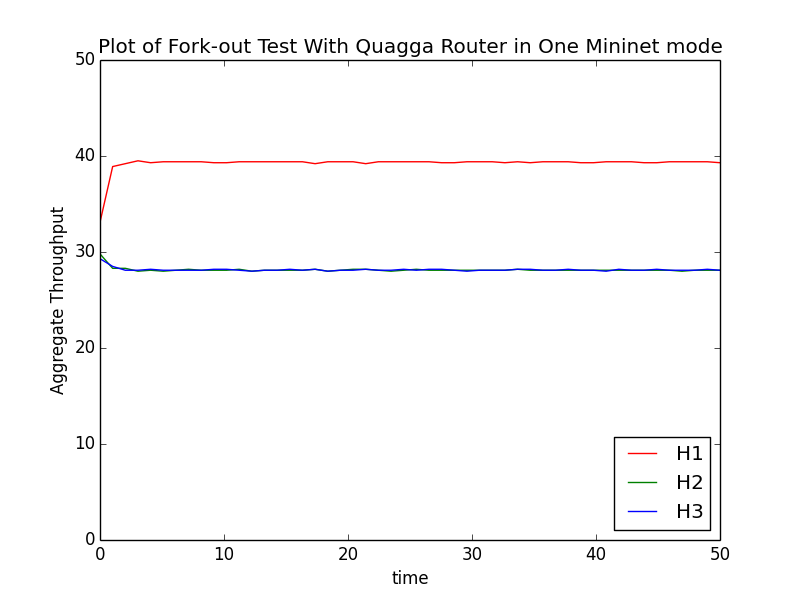
\includegraphics[width=0.6\textwidth]{./Figure/OneMininet(SDN+NONSDN)/ForkOut/ForkOut.png}
\end{figure}

\subsection{Two Mininet}\label{two-mininet}

\subsubsection{Two-way Topology(Two Mininet):}\label{two-way-topologytwo-mininet}

We put two-way test components in two mininet by spliting the one
mininet topology symmetrically. The goal is to prove a substitution of
virtual link into physical link will not make performance down.

\begin{figure}[h]
\centering
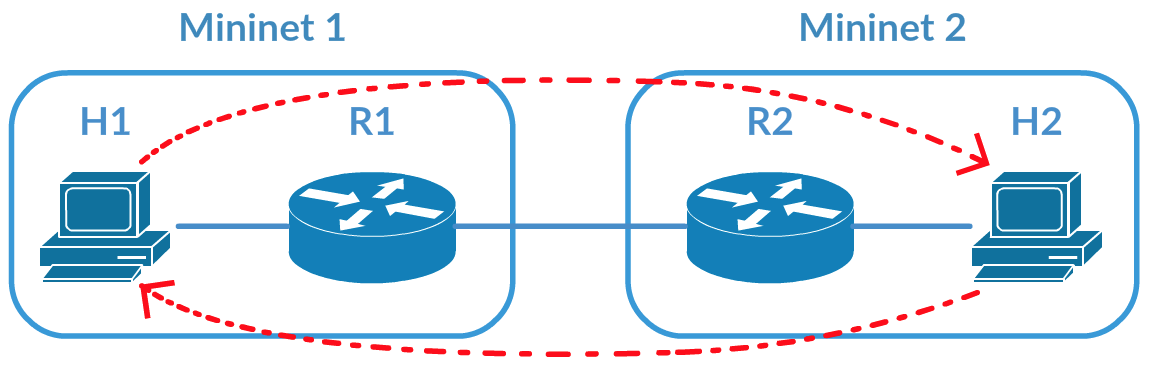
\includegraphics[width=0.7\textwidth]{./Figure/Hybrid/TwoWay/Twoway(TwoMininet).png}
\caption{Two-way Topology(Two Mininet) \label{fig:Two-way Topology(Two Mininet)}}
\end{figure}

\begin{figure}[h]
\centering
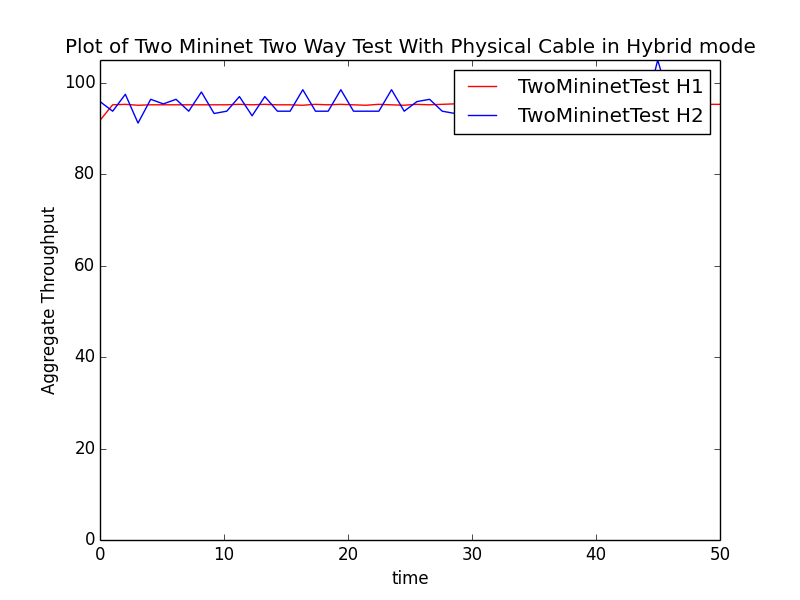
\includegraphics[width=0.6\textwidth]{./Figure/Hybrid/TwoWay/TwoMininetPlot.png}
\end{figure}

\subsection{Hybrid}\label{hybrid}

\subsubsection{Two-way Topology(Add Pica8):}\label{two-way-topologyadd-pica8}

There are 2 aspects that need to be evaluated in Hybrid mode: the
physical port and Pica8 switch. By introducing non-SDN components into
SDN network topology, we made our testbed capable of emulating
traditional network experiment other than SDN network experiment. With
both virtual and physical components inside, we have maintain the
fidelity as well as scalability and reproducibility.


\begin{figure}[h]
\centering
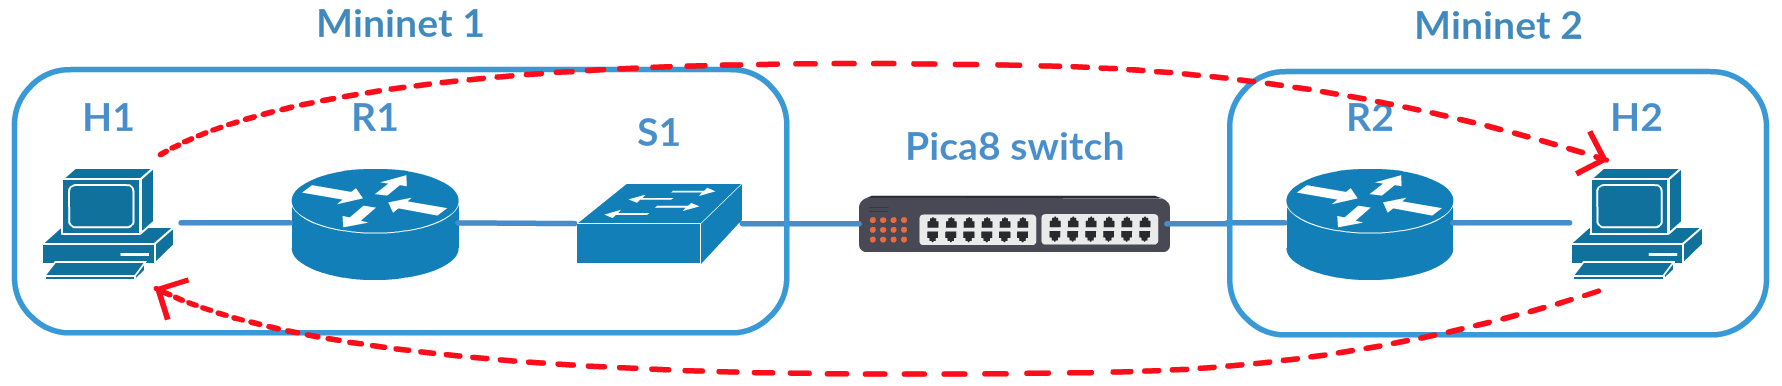
\includegraphics[width=0.7\textwidth]{./Figure/Hybrid/AddPica8/AddPica8(Hybrid).png}
\caption{Two-way Topology(Add Pica8) \label{fig:Two-way Topology(Add Pica8)}}
\end{figure}

\begin{figure}[h]
\centering
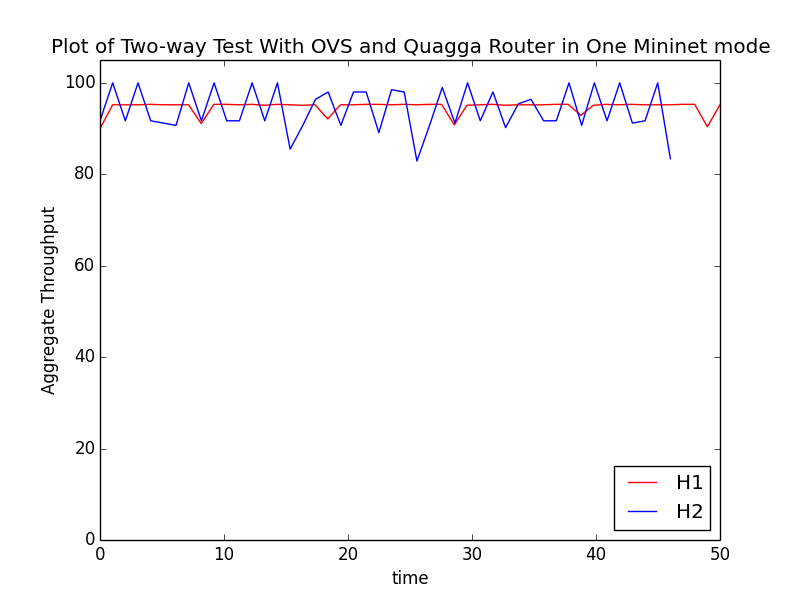
\includegraphics[width=0.6\textwidth]{./Figure/Hybrid/AddPica8/AddPica8.png}
\end{figure}
